\documentclass[12pt,letterpaper,USenglish]{article}

\usepackage[most]{tcolorbox}
\usepackage{amsmath}
\usepackage{amssymb}
\usepackage{microtype}
\usepackage{tikz}
\usepackage{paralist}
\usetikzlibrary{calc,positioning,backgrounds,intersections,graphdrawing,shapes,graphs,arrows,arrows.meta,chains}
\usegdlibrary{trees}

%%% Please use define.org for macros.
\input{define.orgtex}

\begin{document}

\newcommand{\rempos}[1]{%
  \begin{tikzpicture}[remember picture,overlay]
    \node (#1) {};
  \end{tikzpicture}}

\tikzset{lead/.style={anchor=north west,font=\it\bfseries,text=algs4red},
  treenode/.style={draw, minimum
      height=13pt, fill=white,inner sep=3pt, font=\footnotesize,
      rounded rectangle},
    algs4arrow/.style={->,>={Latex[length=7pt]},line width=0.8mm,algs4red},
    graphs/mytree/.style= {
    tree layout,
    sibling distance=5mm, level distance=5mm,
    nodes={treenode},
    edges={thick}},
  gnode/.style={draw,circle,treenode,font=\ttfamily\footnotesize},
  algs4arrow/.style={->,>={Latex[length=7pt]},line width=0.8mm,algs4red},
  redlink/.style = {algs4red, line width=3pt},
  heading/.style = {text width=20cm, fill=algs4red,text=white, align=left,
  font=\sffamily\bfseries}}


\def\mm#1{\text{\small\normalfont\color{algs4red}\itshape\ensuremath{#1}}}
\def\myto{\mm{\to}}
\def\t#1{\texttt{\color{algs4red}#1}}

\newsavebox{\codebox}% For saving code
\begin{lrbox}{\codebox}
\begin{lstalgs4}
     public class |Graph|
$\rlap{\rule[15pt]{15cm}{.3pt}}$                  Graph(int V)           @$\myto$ new $\t{V}$-vertex, $\t{0}$-edge graph
              int V(), E()               @$\myto$ number of vertices/edges
             void addEdge(int v, int w)  @$\myto$ add edge $\t{v-w}$
Iterable<Integer> adj(int v)             @$\myto$ vertices adjacent to $\t{v}$
\end{lstalgs4}
\end{lrbox}


\noindent\begin{tikzpicture}[every node/.style={anchor=north west},remember picture]
  % Main background
  \begin{scope}[on background layer]
    \fill[black!10!white, draw=white, line width=6pt] (-.5\textwidth, 0) rectangle (.5\textwidth, -18cm);
  \end{scope}

  % Clip and left margin
  \path [save path=\theframe, rounded corners] ($(-.5\textwidth, 0) + (1.5pt,-1.5pt)$)
  rectangle ($(.5\textwidth, -18cm) + (-1.5pt, 1.5pt)$);
  \clip [use path=\theframe];
  \coordinate (left) at ($(-.5\textwidth, 0) + (0.3cm,0)$);

  % Title
  \node [anchor=north,text width=20cm,minimum height=1.4cm,align=center,fill=algs4red,text=white]
  {\sffamily\Large \textbf{4.2}\quad DIRECTED GRAPHS: PART I};

  % Definition
  \node [lead] (def) at (left |- 0, -1.6cm) {Definition.};%
  \node [right=0cm of def] {A set of \emph{vertices} (nodes) and a collection of
    \emph{directed edges} that
    connect ordered pairs of vertices.};

  %% Glossary lead
  \node [heading] (glos) at (-.5\textwidth,-2.5cm) {~~Directed acyclic graphs
    (DAG) and topological sorts};

  \def\mph#1{\emph{\color{algs4red}#1}}
  \node (x) at ($(glos.south west) + (-.2cm, -.2cm)$) {\begin{minsizebox}{19cm}{10cm}
      \begin{compactitem}
      \item \mph{Detecting cycles:} depth-first search and check for cycles
        \emph{on the stack}.\\[.4cm]
        \hspace{3cm}{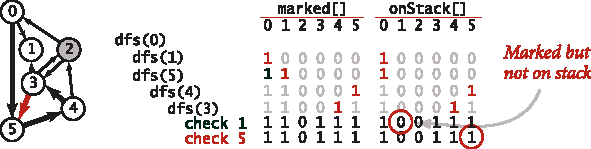
\includegraphics[height=3cm]{dfscycle}}
        \vspace{.3cm}
      \item \mph{Topological order:} ordering of the vertices of a DAG such that
        if \lstinline{u$\leadsto$v}, then \lstinline{u} appears before \lstinline{v}.
        \\[.4cm]
        \centerline{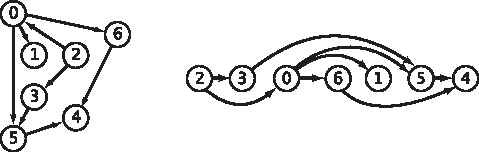
\includegraphics[height=3cm]{toposort}} \vspace{.3cm}
      \item \mph{Pre-topological order:} an ordering of a \emph{digraph} such
        that if \lstinline{u$\leadsto$v} \emph{and not} \lstinline{v$\leadsto$u}, then
        \lstinline{u} appears before \lstinline{v}.
      \item \mph{Computing (pre-)topological order:} take the \emph{reverse postorder}
        of a \emph{complete} DFS on the graph, that is, the reverse of the nodes seen
        after the recursive calls to DFS.
      \end{compactitem}
    \end{minsizebox}};

  \node[fill=algs4red!40, inner sep=0.3cm, anchor=north] at ($(x.south west -|
  0cm, 0cm) + (0, -.2cm)$)  {
    % \begin{minsizebox}{16cm}{3cm}
    %   \textbf{Lemma.} Let \(C\) be a strong component (see next card) of a graph
    %   \(G\) and \lstinline{v} a vertex not in \(C\).  If there is a path from
    %   \lstinline{v} to \(C\), then \lstinline{v} appears before \emph{every}
    %   vertex in \(C\) in the reverse postorder of \(G\).\\[4pt]

    %   \textbf{Proof.} If \lstinline{v} is visited before every vertex in \(C\),
    %   then every vertex in \(C\) will be visited and finished before \lstinline{v}
    %   finishes. If some vertex in \(C\) is visited before \lstinline{v}, then all
    %   vertices in \(C\) will be visited and finished before \lstinline{v} is
    %   visited, because \lstinline{v} is not reachable from any vertex in \(C\).
    % \end{minsizebox}
    \begin{minsizebox}{16cm}{3.3cm}
      \textbf{Lemma.} Let \lstinline{u} and \lstinline{v} be vertices such that
      \lstinline{u$\leadsto$v} \emph{and not} \lstinline{v$\leadsto$u}, then \lstinline{u}
      appears before
      \lstinline{v} in the reverse postorder of \(G\).  In other words, the
      reverse postorder is a pre-topological order.\\[4pt]

      \textbf{Proof.} If \lstinline{u} is visited before \lstinline{v},
      then \lstinline{v} will be finished before \lstinline{u}
      finishes, hence \lstinline{u} will appear before \lstinline{v} in the
      reverse postorder.  If \lstinline{v} is visited before \lstinline{u}, then
      \lstinline{v} has to be finished before visiting \lstinline{u}, since
      \lstinline{u} is not reachable from \lstinline{v}.  Again, \lstinline{u}
      will appear before \lstinline{v} in the reverse postorder.
    \end{minsizebox}
  };
    %% implem

  %% Box
  \draw [algs4red,line width=3pt] [use path=\theframe];

\end{tikzpicture}
\end{document}
